\documentclass[a4paper, 12pt]{article}
\usepackage[T2A]{fontenc}
\usepackage[utf8]{inputenc}
\usepackage[english,russian]{babel}
\usepackage{amsmath, amsfonts, amssymb, amsthm, mathtools}
\usepackage{graphicx}
\usepackage{float}
\usepackage{wrapfig}
\usepackage{subfigure}

\author{Легких Никита\\
Группа Б05-301}
\title{{\bf{\hugeОтчет о выполнении лабораторной работы 2.3.1}}\\[10pt]
Получение и измерение вакуума}
\date{}

\begin{document}
\maketitle
\newpage
\section{Введение}
\textbf{Цель работы:} 1) Измерение объемов форвакуумной и высоковакуумной частей установки; 2) Определение скорости откачки системы в стационарном режиме, а также по ухудшению и улучшению вакуума.\\
\textbf{В работе используются:} Вакуумная установка с манометрами: масляным, термопарным и ионизационным.

\section{Теоретическая справка}
\subsection{Экспериментальная установка}
 В данной работе используются традиционные методы откачки механическим форвакуумным насосом до давления $10^{-2}$ торр и диффузионным масляным насосом до давления $10^{-4}$ торр. \\
 Установка изготовлена из стекла, и состоит из форвакуумного баллона (ФБ), высоковакуумного диффузионного насоса (ВН), высоковакуумного баллона (ВБ), масляного (М) и ионизационного (И) манометров, термопарных манометров ($\text{М}_1$ и $\text{М}_2$), форвакуумного насоса (ФН) и соединительных кранов ($K_1, K_2,..., K_6$) (рис. 1). Кроме того, в состав установки входят: вариатор (автотрансформатор с регулируемым выходным напряжением), или реостат и амперметр для регулирования тока нагревателя диффузионного насоса. \\
  \begin{figure}[!h]
   \centering
   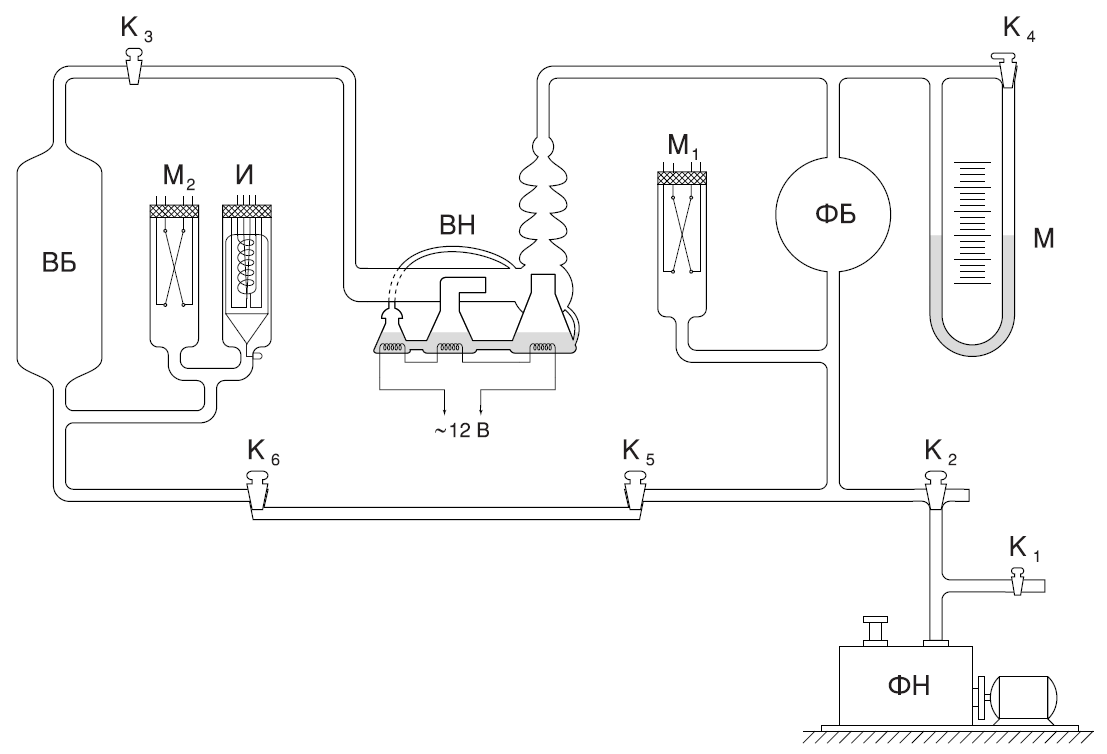
\includegraphics[width=0.5\linewidth]{2.3.1/Схема установки.PNG}
   \caption[]{Схема установки}
   \label{fig:Схема установки}
 \end{figure}
 Все краны вакуумной установки стеклянные. Стенки кранов тонкие, пробки кранов полые и составляют одно целое с рукоятками. Пробки кранов притерты к корпусам. Для герметизации используется вакуумная смазка. \\
 Устройство и принцип действия \textit{форвакуумного насоса} схематически, но довольно ясно изображены на рис 2. В положениях <<а>> и <<б>> пластина <<А>> засасывает разреженный воздух из откачиваемого объёма, а пластина <<Б>> вытесняет ранее захваченный воздух в атмосферу. В положениях <<в>> и <<г>> пластины поменялись ролями.
\begin{figure}[!h]
  \centering
  \includegraphics[width=0.9\linewidth]{2.3.1/Устройство фв насоса.PNG}
  \caption[]{Схема действия ротационного двухпластинчатого форвакуумного насоса}
  \label{fig:Схема ФВ насоса}
\end{figure}
Устройство и принцип действия \textit{диффузионного насоса} схематически изображены на рис 2. Такой насос работает в тысячи раз быстрее форвакуумного. Его действие основано на диффузии. Масло, налитое в сосуд А, подогревается электрической печкой. Пары масла поднимаются по трубке Б и вырываются из сопла В. Струя паров увлекает молекулы газа, которые поступают из откачиваемого сосуда через трубку ВВ. В трубке Г мало осаждается и стекает вниз. Оставшийся газ, выходя в трубку ФВ, откачивается форвакуумным насосом. \\
Диффузионный насос работает наиболее эффективно, когда длина свободного пробега молекул примерно равна ширине кольцевого зазора между соплом В и стенками трубки ВВ. Давление насыщенных паров масла при рабочей температуре, создаваемой обогревателем сосуда А, много больше $5\cdot 10^{-2}$ торр, поэтому пары масла создают плотную струю, увлекающую с собой молекулы газа.
\begin{figure}[!h]
  \centering
  \includegraphics[width=0.4\linewidth]{2.3.1/Устройство вв насоса.PNG}
  \caption[]{Схема работы диффузионного насоса}
  \label{fig:Схема ВВ насоса}
\end{figure}

 Диффузионный насос, используемый в нашей установке (см. рис 1) имеет две ступени и соответственно два сопла. Одно сопло вертикальное (первая ступень), второе горизонтальное (вторая ступень). За второй ступенью имеется ещё одна печь, но пар из этой печи поступает не в сопло, а по тонкой трубке подводится ближе к печке первой ступени. Эта печь осуществляет фракционирование масла. Легколетучие фракции масла, испаряясь, поступают в первую ступень, обогащая её. По этой причине плотность струи первой ступени выше, и эта ступень начинает откачивать при более высоком давлении в форвакуумной части. Вторая ступень обогащается малолетучими фракциями масла. Плотность струи второй ступени меньше, но меньше и давление насыщенных паров. Соответственно, в откачиваемый объем поступает меньше паров масла, и его удаётся откачать до более высокого вакуума.
 \begin{wrapfigure}{r}{50mm}
   \begin{center}
     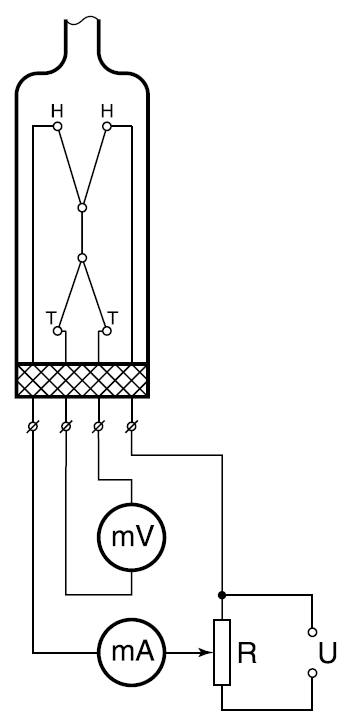
\includegraphics[width=0.9\linewidth]{2.3.1/термопара.PNG}
     \caption{Схема термопарного манометра с лампой ЛТ-2}
     \label{fig:Схема термопары}
   \end{center}
 \end{wrapfigure}
 \textit{Термопарный манометр.} Чувствительным элементом манометра является платиново-родиевая термопара, спаянная с никелевой нитью накала и заключённая в стеклянный баллон. Устройство термопары пояснено на рис. 4. По нити накала НН пропускается ток постоянной величины. Для установки тока служит потенциометр R, расположенный на передней панели вакуумметра. Термопара ТТ присоединяется к милливольтметру, показания которого определяются температурой нити накала и зависят от отдачи тепла в окружающее пространство. \\
 Потери тепла определяются теплопроводностью нити и термопары, теплопроводностью газа, переносом тепла конвективными потоками газа внутри лампы, и теплоизлучением нити (инфракрасное тепловое излучение). В обычном режиме лампы основную роль играет теплопроводность газа. При давлениях, не меньших 1 торр, теплопроводность газа, а вместе с ней и ЭДС термопары практически не зависят от давления газа, и прибор не работает. \\
 При улучшении вакуума средний свободный пробег молекул становится сравнимым с диаметром нити, теплоотвод падает, и температура спая возрастает. При вакууме порядка $10^{-3}$ торр теплоотвод, осуществляемый газом, становится сравнимым с другими потерями тепла, и температура становится практически постоянной. Градуировочная кривая термопары приведена на рис. 5.
\begin{figure}[!h]
   \centering
   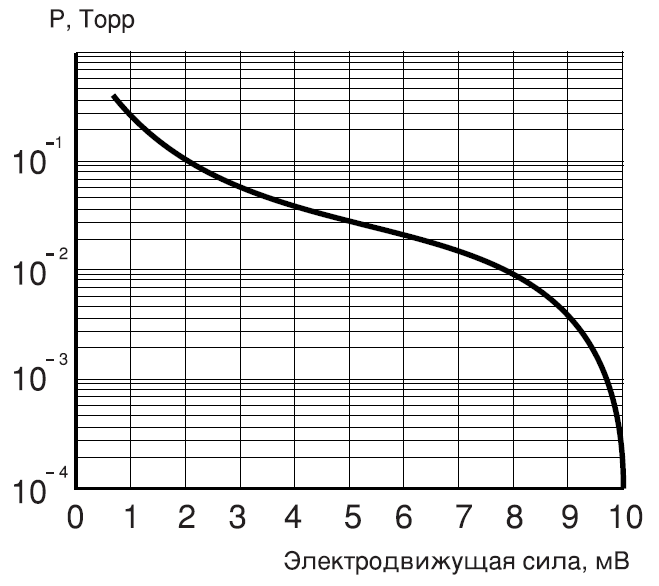
\includegraphics[width=0.5\linewidth]{2.3.1/градуировочная кривая.PNG}
   \caption[]{Градуировочная кривая термопары ЛТ-2}
   \label{fig:Градуировочная кривая}
\end{figure}
\newpage
\begin{wrapfigure}{r}{60mm} %если не лезет, но с новой стр
  \begin{center}
    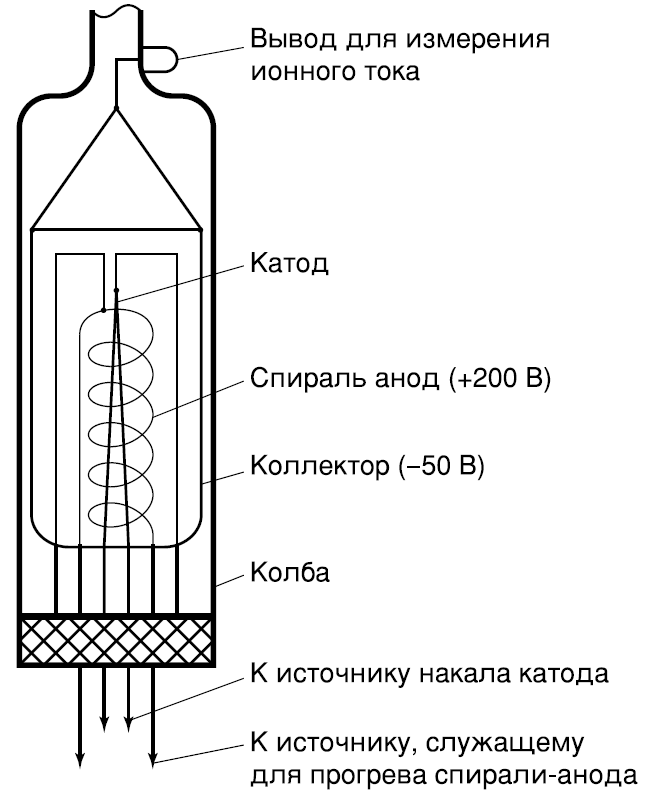
\includegraphics[width=60mm]{2.3.1/лампа.PNG}
    \caption{Схема ионизационной лампы ЛТ-2}
    \label{fig:лампа}
  \end{center}
\end{wrapfigure}
\textit{Ионизационный манометр.} Схема ионизационного манометра изображения на рисунке 6. Он представляет собой трехэлектродную лампу. Электроны испускаются раскалённым катодом и увлекаются электрическим полем к аноду, имеющему вид редкой спирали. Проскакивая за её витки, электроны замедляются полем коллектора и возвращаются к аноду. Прежде чем осесть на аноде, они успевают много раз пересечь пространство между катодом и коллектором. На своём пути электроны ионизуют молекулы газа. Ионы, образовавшиеся между анодом и коллектором, притягиваются полем коллектора и определяют его ток. \\
Накалённый катод ионизационного манометра перегорает, если давление в системе превышает $10^{-3}$ торр, поэтому перед его включением необходимо проверить давление термопарным манометром. \\
\subsection{Процесс откачки}
Опишем процесс откачки математически: \\
Пусть W --- объем газа, удаляемого из сосуда при данном давлении за единицу времени, $Q_i$ для различных значений i обозначим различные притоки газа в сосуд (в единицах $PV$), такие как течи извне $Q_\text{и}$, десорбция с поверхностей внутри сосуда $Q_\text{д}$, обратный ток через насос $Q_\text{н}$. Тогда, приравнивая убыль газа из сосуда (с точностью до $RT/\mu$) в единицу времени $-VdP$ и сумму перечисленных токов? имеем:

 \begin{equation}
   -VdP = (PW - \sum_i Q_i)dt
 \end{equation}
 При достижении предельного вакуума устанавливается давление $P_{\text{пр}}$, и $dP = 0$. Тогда
 \begin{equation}
    W = ( \sum_i Q_i )/P_{\text{пр}}
 \end{equation}
 Поскольку обычно $Q_\text{и}$ постоянно, а $Q_\text{н}$ и $Q_\text{д}$ слабо зависят от времени, также считая постоянной W, можем проинтегрировать (1) и получить:
 \begin{equation}
   P - P_{\text{пр}} = (P_0 - P_{\text{пр}})\exp(-\frac{W}{V}t)
 \end{equation}
Полная скорость откачки $W$, собственная скорость откачки насоса $W_{\text{н}}$ и проводимости элементов системы $C_1, C_2,...$ соотносятся согласно формуле (4), и это учтено в конструкции установки.
 \begin{equation}
 \frac{1}{W} = \frac{1}{W} + \frac{1}{C_1} + \frac{1}{C_2} + ...
\end{equation}

\subsection{Течение газа через трубу}
Характер течения газа существенно зависит от соотношения между размерами системы и длиной свободного пробега молекул. При атмосферном и форвакуумном давлениях  длина свободного пробега меньше диаметра трубок, и течение газа определяется его вязкостью, т.е. взаимодействием молекул. При высоком вакууме течение существеннее определяется взаимодействием со стенками \\
Для количества газа, протекающего через трубу длины $l$ и радиуса $r$ в условиях высокого вакуума, справедлива формула:
\begin{equation}
  \frac{d(PV)}{dt} = \frac{4}{3}r^3\sqrt{\frac{2\pi RT}{\mu}}\frac{P_2 - P_1}{l}
\end{equation}
Если труба соединяет насос установку, то давлением $P_1$ у насоса можно пренебречь. Давление в сосуде $P = P_2$. Тогда имеем:
\begin{equation}
C_\text{тр} = \left(\frac{dV}{dt}\right)_\text{тр} = \frac{4r^3}{3l}\sqrt{\frac{2\pi RT}{\mu}}
\end{equation}
Для пропускной способности отверстий имеется формула
\begin{equation}
C_\text{отв} = \left(\frac{dV}{dt}\right)_\text{отв} = S\frac{\bar{\upsilon}}{4}
\end{equation}
Для воздуха при комнатной температуре $\bar{\upsilon}/4 = 110~\text{м/с} = 11~\text{л/c}\cdot\text{см}^2$.
\section{Результаты измерений и обработка данных}
\subsection{Изменений объемов форвакуумной и высоковакуумной частей установки}
В начале работы запишем параметры установки:\\
$\rho_{масл} = 0,885$ $\frac{\text{г}}{\text{см}^3}$\\
$V_{\text{к6+к5+кап}}= 50$ $\text{см}^3$\\
$L = 10,8$ $\text{см}$\\
$d_{\text{кап}} = 0,8$ $\text{см}$\\
Далее определим объемы форвакуумной и высоковакуумной частей установки по методу, описанному в задании. Результаты измерений составили:\\
$\Delta h_1 = 35 - 9,3 = 25,7$ $\text{см}$, $\sigma_{\Delta h_1} = 0,2$ $\text{см}$\\
$\Delta h_2 = 30,6 - 14,2 = 16,4$ $\text{см}$, $\sigma_{\Delta h_2} = 0,2$ $\text{см}$\\
Заметим при этом, что измерения были проведены дважды и в каждом случае результат отличался в пределах погрещностей.\\
Зная объем "запертой" части установки $V_{\text{к6+к5+кап}} = 50$ $\text{см}^3$ и используя закон Бойля-Мариота $P_\text{1} V_{\text{к6+к5+кап}} = P_2 V_{\text{фв}}$, вычислим объем форвакуумной части установки. При этом давление $P_1 = P_{атм} = (98.4 \pm 0.1)$ $\text{кПа}$, $P_2 =   \rho_{масл} g \Delta h_1$, а относительная погрешность полученного значения равна:\\
$\varepsilon_{V_{\text{фв}}} = \sqrt{\varepsilon_{\Delta h_1}^2 + \varepsilon_{P_1}^2}$.\\
В результате имеем: 
\begin{equation}
    V_{\text{фв}} = (2,21 \pm 0,02) \text{ л}
\end{equation}
Проведем аналогичные измерения, запустив воздух и в высоковауукумную часть, найдем их общий объем:\\
\begin{equation}
    V_{\text{фв+вв}} = (3,46 \pm 0,04) \text{ л}
\end{equation}
Тогда:
\begin{equation}
    V_{\text{вв}} = V_{\text{фв+вв}} - V_{\text{фв}} = (1,25 \pm 0,06) \text{ л}
\end{equation}
\subsection{Получение высокого вакуума и измерение скорости откачки}
Перейдем к получению высокого вакуума. Следуя инструкции, получим предельное давление:\\
$P_{\text{пр}} = 6,6 \cdot 10^{-5}$ $\text{торр}$\\
Далее проведем измерения по ухудшению и улучшению вакуума во время откачки:
Улучшение:
\begin{table}[H]
\begin{tabular}{|ccc|ccc|}
\hline
\multicolumn{3}{|c|}{Измерение 1}                             & \multicolumn{3}{c|}{Измерение 2}                            \\ \hline

\multicolumn{1}{|c|}{$t$, с}  & \multicolumn{1}{c|}{$P$, торр $\cdot 10^{-5}$}   & \multicolumn{1}{c|}{$ln(P-P_{\text{пр}})$} & \multicolumn{1}{|c|}{$t$, с}  & \multicolumn{1}{c|}{$P$, торр $\cdot 10^{-5}$}   & \multicolumn{1}{c|}{$ln(P-P_{\text{пр}})$} \\ \hline
\multicolumn{1}{|c|}{0}  & \multicolumn{1}{c|}{70}  & 4,1495  & \multicolumn{1}{c|}{0}  & \multicolumn{1}{c|}{70} & 4,1495  \\ \hline
\multicolumn{1}{|c|}{1}  & \multicolumn{1}{c|}{69}  & 4,1336  & \multicolumn{1}{c|}{1}  & \multicolumn{1}{c|}{69} & 4,1336  \\ \hline
\multicolumn{1}{|c|}{2}  & \multicolumn{1}{c|}{66}  & 4,0843  & \multicolumn{1}{c|}{2}  & \multicolumn{1}{c|}{63} & 4,0325  \\ \hline
\multicolumn{1}{|c|}{3}  & \multicolumn{1}{c|}{59}  & 3,9589  & \multicolumn{1}{c|}{3}  & \multicolumn{1}{c|}{55} & 3,8795  \\ \hline
\multicolumn{1}{|c|}{4}  & \multicolumn{1}{c|}{50}  & 3,7705  & \multicolumn{1}{c|}{4}  & \multicolumn{1}{c|}{46} & 3,6738  \\ \hline
\multicolumn{1}{|c|}{5}  & \multicolumn{1}{c|}{40}  & 3,5086  & \multicolumn{1}{c|}{5}  & \multicolumn{1}{c|}{37} & 3,4144  \\ \hline
\multicolumn{1}{|c|}{6}  & \multicolumn{1}{c|}{32}  & 3,2347  & \multicolumn{1}{c|}{6}  & \multicolumn{1}{c|}{30} & 3,1527  \\ \hline
\multicolumn{1}{|c|}{7}  & \multicolumn{1}{c|}{26}  & 2,9653  & \multicolumn{1}{c|}{7}  & \multicolumn{1}{c|}{25} & 2,9124  \\ \hline
\multicolumn{1}{|c|}{8}  & \multicolumn{1}{c|}{22}  & 2,7344  & \multicolumn{1}{c|}{8}  & \multicolumn{1}{c|}{21} & 2,6672  \\ \hline
\multicolumn{1}{|c|}{9}  & \multicolumn{1}{c|}{19}  & 2,5177  & \multicolumn{1}{c|}{9}  & \multicolumn{1}{c|}{18} & 2,4336  \\ \hline
\multicolumn{1}{|c|}{10} & \multicolumn{1}{c|}{17}  & 2,3418  & \multicolumn{1}{c|}{10} & \multicolumn{1}{c|}{16} & 2,2407  \\ \hline
\multicolumn{1}{|c|}{11} & \multicolumn{1}{c|}{15}  & 2,1282  & \multicolumn{1}{c|}{11} & \multicolumn{1}{c|}{15} & 2,1282  \\ \hline
\multicolumn{1}{|c|}{12} & \multicolumn{1}{c|}{13}  & 1,8563  & \multicolumn{1}{c|}{12} & \multicolumn{1}{c|}{13} & 1,8563  \\ \hline
\multicolumn{1}{|c|}{13} & \multicolumn{1}{c|}{12}  & 1,6864  & \multicolumn{1}{c|}{13} & \multicolumn{1}{c|}{12} & 1,6864  \\ \hline
\multicolumn{1}{|c|}{15} & \multicolumn{1}{c|}{11}  & 1,4816  & \multicolumn{1}{c|}{14} & \multicolumn{1}{c|}{11} & 1,4816  \\ \hline
\multicolumn{1}{|c|}{17} & \multicolumn{1}{c|}{9,8} & 1,1632  & \multicolumn{1}{c|}{16} & \multicolumn{1}{c|}{10} & 1,2238  \\ \hline
\end{tabular}
\caption{Измерения при улучшении вакуума}
\end{table}
На основании полученных данных построим графики:
\begin{figure}[H]
    \begin{center}
    
\includegraphics[width=0.6\linewidth]{2.3.1/1граф.png}
    \end{center}
  \caption{Зависимость давления от времени при улучшении вакуума (измерение 1)}
\end{figure}
\begin{figure}[H]
    \begin{center}
    
\includegraphics[width=0.6\linewidth]{2.3.1/2граф.png}
    \end{center}
  \caption{Зависимость давления от времени при улучшении вакуума (измерение 2)}
\end{figure}
\noindent С помощью МНК найдем коэффициенты наклона графиков:\\
$k_1 = - (0,199 \pm 0,007)$ $\text{c}^{-1}$\\
$k_2 = - (0,203  \pm 0,005)$ $\text{c}^{-1}$\\
Во-первых, заметим, что значения совпадают в пределах погрешностей. Во-вторых, найдем их среднее:\\
$k = - (0,201 \pm 0,009)$ $\text{c}^{-1}$\\
Теперь, зная коэффициент наклона графика, найдем $W$:\\
$W = -kV_{вв} = (0,251 \pm 0,016)$ л/c.\\
\newpage
Далее проведем измерения по ухудшению вакуума:
\begin{table}[H]
\begin{tabular}{|cccc|ccll|}
\hline
\multicolumn{4}{|c|}{Измерение 1}                                                                      & \multicolumn{4}{c|}{Измерение 2}                                                                        \\ \hline
\multicolumn{1}{|c|}{$t$, c}  & \multicolumn{1}{c|}{$P$, торр $\cdot 10^{-5}$}   & \multicolumn{1}{|c|}{$t$, c}   & $P$, торр $\cdot 10^{-5}$                     & \multicolumn{1}{c|}{$t$, c}  & \multicolumn{1}{c|}{$P$, торр $\cdot 10^{-5}$}   & \multicolumn{1}{c|}{$t$, c}   & \multicolumn{1}{c|}{$P$, торр $\cdot 10^{-5}$}   \\ \hline

\multicolumn{1}{|c|}{0}  & \multicolumn{1}{c|}{6,6} & \multicolumn{1}{c|}{65}  & 39                    & \multicolumn{1}{c|}{0}  & \multicolumn{1}{c|}{7,7} & \multicolumn{1}{c|}{65}  & \multicolumn{1}{c|}{44} \\ \hline
\multicolumn{1}{|c|}{5}  & \multicolumn{1}{c|}{7,1} & \multicolumn{1}{c|}{70}  & 42                    & \multicolumn{1}{c|}{5}  & \multicolumn{1}{c|}{9,5} & \multicolumn{1}{c|}{70}  & \multicolumn{1}{c|}{47} \\ \hline
\multicolumn{1}{|c|}{10} & \multicolumn{1}{c|}{8,6} & \multicolumn{1}{c|}{75}  & 45                    & \multicolumn{1}{c|}{10} & \multicolumn{1}{c|}{13}  & \multicolumn{1}{c|}{75}  & \multicolumn{1}{c|}{49} \\ \hline
\multicolumn{1}{|c|}{15} & \multicolumn{1}{c|}{10}  & \multicolumn{1}{c|}{80}  & 47                    & \multicolumn{1}{c|}{15} & \multicolumn{1}{c|}{16}  & \multicolumn{1}{c|}{80}  & \multicolumn{1}{c|}{52} \\ \hline
\multicolumn{1}{|c|}{20} & \multicolumn{1}{c|}{14}  & \multicolumn{1}{c|}{85}  & 50                    & \multicolumn{1}{c|}{20} & \multicolumn{1}{c|}{19}  & \multicolumn{1}{c|}{85}  & \multicolumn{1}{c|}{55} \\ \hline
\multicolumn{1}{|c|}{25} & \multicolumn{1}{c|}{16}  & \multicolumn{1}{c|}{90}  & 52                    & \multicolumn{1}{c|}{25} & \multicolumn{1}{c|}{22}  & \multicolumn{1}{c|}{90}  & \multicolumn{1}{c|}{57} \\ \hline
\multicolumn{1}{|c|}{30} & \multicolumn{1}{c|}{19}  & \multicolumn{1}{c|}{95}  & 55                    & \multicolumn{1}{c|}{30} & \multicolumn{1}{c|}{25}  & \multicolumn{1}{c|}{95}  & \multicolumn{1}{c|}{59} \\ \hline
\multicolumn{1}{|c|}{35} & \multicolumn{1}{c|}{23}  & \multicolumn{1}{c|}{100} & 58                    & \multicolumn{1}{c|}{35} & \multicolumn{1}{c|}{28}  & \multicolumn{1}{c|}{100} & \multicolumn{1}{c|}{62} \\ \hline
\multicolumn{1}{|c|}{40} & \multicolumn{1}{c|}{26}  & \multicolumn{1}{c|}{105} & 60                    & \multicolumn{1}{c|}{40} & \multicolumn{1}{c|}{31}  & \multicolumn{1}{c|}{105} & \multicolumn{1}{c|}{65} \\ \hline
\multicolumn{1}{|c|}{45} & \multicolumn{1}{c|}{29}  & \multicolumn{1}{c|}{110} & 62                    & \multicolumn{1}{c|}{45} & \multicolumn{1}{c|}{34}  & \multicolumn{1}{c|}{110} & \multicolumn{1}{c|}{67} \\ \hline
\multicolumn{1}{|c|}{50} & \multicolumn{1}{c|}{31}  & \multicolumn{1}{c|}{115} & 65                    & \multicolumn{1}{c|}{50} & \multicolumn{1}{c|}{36}  & \multicolumn{1}{c|}{115} & \multicolumn{1}{c|}{69} \\ \hline
\multicolumn{1}{|c|}{55} & \multicolumn{1}{c|}{34}  & \multicolumn{1}{c|}{120} & 67                    & \multicolumn{1}{c|}{55} & \multicolumn{1}{c|}{39}  & \multicolumn{1}{c|}{120} & \multicolumn{1}{c|}{71} \\ \hline
\multicolumn{1}{|c|}{60} & \multicolumn{1}{c|}{37}  & \multicolumn{1}{c|}{125} & 70                    & \multicolumn{1}{c|}{60} & \multicolumn{1}{c|}{42}  & \multicolumn{1}{l|}{}    &                         \\ \hline
\end{tabular}
\caption{Измерения при ухудшению вакуума}
\end{table}
Отразим полученные результаты на графиках:
\begin{figure}[H]
    \begin{center}
    
\includegraphics[width=0.6\linewidth]{2.3.1/3граф.png}
    \end{center}
  \caption{Зависимость давления от времени при ухудшении вакуума (измерение 1)}
\end{figure}
\begin{figure}[H]
    \begin{center}
    
\includegraphics[width=0.6\linewidth]{2.3.1/4граф.png}
    \end{center}
  \caption{Зависимость давления от времени при ухудшении вакуума (измерение 2)}
\end{figure}
\noindent С помощью МНК найдем коэффициенты наклона графиков:\\
$k_1 = (0,531 \pm 0,005)$ $\cdot 10^{-5} \text{торр} \cdot \text{c}^{-1}$\\
$k_2 = (0,536 \pm 0,005)$ $\cdot 10^{-5} \text{торр} \cdot \text{c}^{-1}$\\
Во-первых, заметим, что значения совпадают в пределах погрешностей. Во-вторых, найдем их среднее:\\
$k = (0,534 \pm 0,007)$ $\cdot 10^{-5} \text{торр} \cdot \text{c}^{-1}$\\
С помощью полученных результатов оценим величину потока $Q_{\text{н}}$:\\
$Q_{\text{н}} = P_{\text{пр}}W - (Q_{\text{д}} + Q_{\text{и}}) = kV_{\text{вв}} = (0,99 \pm 0,08)$ $\cdot 10^{-5} \text{торр} \cdot \text{л/c}$\\

Далее, следуя инструкции, измерим установившееся давление $P_{\text{уст}}$ и давление со стороны форвакуумной части:\\
$P_{\text{уст}} =  1,9 \cdot 10^{-4} \text{торр}$\\
$P_{\text{фв}} =  1 \cdot 10^{-4} \text{торр}$\\
Зная эти результаты, найдем $W$ по следцющим формулам:\\
$$
P_{пр} W = Q_1, \quad P_{уст} W = Q_1 + \frac{d(PV)_{кап}}{dt}, 
$$
$$
\Rightarrow
W = \frac{d(PV)_{\text{кап}}}{dt}\frac{P_{\text{фв}}}{P_{\text{уст}}-P_{\text{пр}}} = (0,279 \pm 0,7) \text{л/c}
$$
\newpage
\section{Выводы}
В ходе работы удалось:
\begin{itemize}
    \item Измерить объемы форвакуумной и высоковакуумной частей установки: $V_{\text{фв}} = (2,21 \pm 0,02) \text{ л}$, $ V_{\text{вв}} = (1,25 \pm 0,06) \text{ л}$ (погрешность измерений меньше 5 \%).
    \item Найти скорость откачки насоса двумя способами:
    \begin{equation*}
        W_{\text{ухудшение вакуума}} = (0,251 \pm 0,016)\text{л/c}; W_{\text{искуственная течь}} = (0,279 \pm 0,7)\text{л/c}
    \end{equation*}
    Полученные значения совпадают в пределах погрешностей, однако видно, что точность второго способа гораздо ниже.
    \item Оценить величину потока: $Q_{\text{н}} = (0,99 \pm 0,08)$ $\cdot 10^{-5} \text{торр} \cdot \text{л/c}$.
\end{itemize}
\end{document}
